\chapter{Inverse Solutions}
\label{ch:inv}

\section{Overview}

The inverse problem of electrocardiography is to find suitable electrical source parameters on the heart that adequately describe the observed body surface potentials. Regularization is typically employed in solution methods to reduce the sensitivity of the problem to relatively small errors in the observed body surface potentials, thereby stabilizing it. As a result, solution methods may be supplied body surface potentials, a forward model, and method-specific regularization parameters as input. Specific use of each method is described below. As output, modules primarily produce the resulting solution with extra outputs, depending on the specific method.

\section{Descriptions of the Inverse Solution Methods Implemented in SCIRun}

%%%%%%%%%%%%%%%%%%%%%%%
\subsection{Tikhonov Regularization}
    
    As described in \autoref{sec:math:standardTikhonov}, Tikhonov regularization is a classical inverse method that solves the following least squares problem:
    \begin{center}
        \begin{eqnarray}
            min_{x} \| P (y - A x) \|^{2}_{2} + \lambda^{2} \| Rx \|^{2}_{2},
        \label{eq:inverseSec_tik_problem}
        \end{eqnarray}
    \end{center}
    where $y$ are the measured ECG potentials, $A$ is the forward matrix, $X$ are the unknown potentials on the heart, $\lambda$ is the regularization parameter, $R$ is a regularization matrix and $P$ is the sensor covariance matrix.
    All these variables can be found as inputs or outputs of the module \href{http://scirundocwiki.sci.utah.edu/SCIRunDocs/index.php/CIBC:Documentation:SCIRun:Reference:BioPSE:SolveInverseProblemWithTikhonov}{{\tt SolveInverseProblemWithTikhonov}}, shown in \autoref{fig:tik_module}.
    \begin{figure}
        \begin{center}
        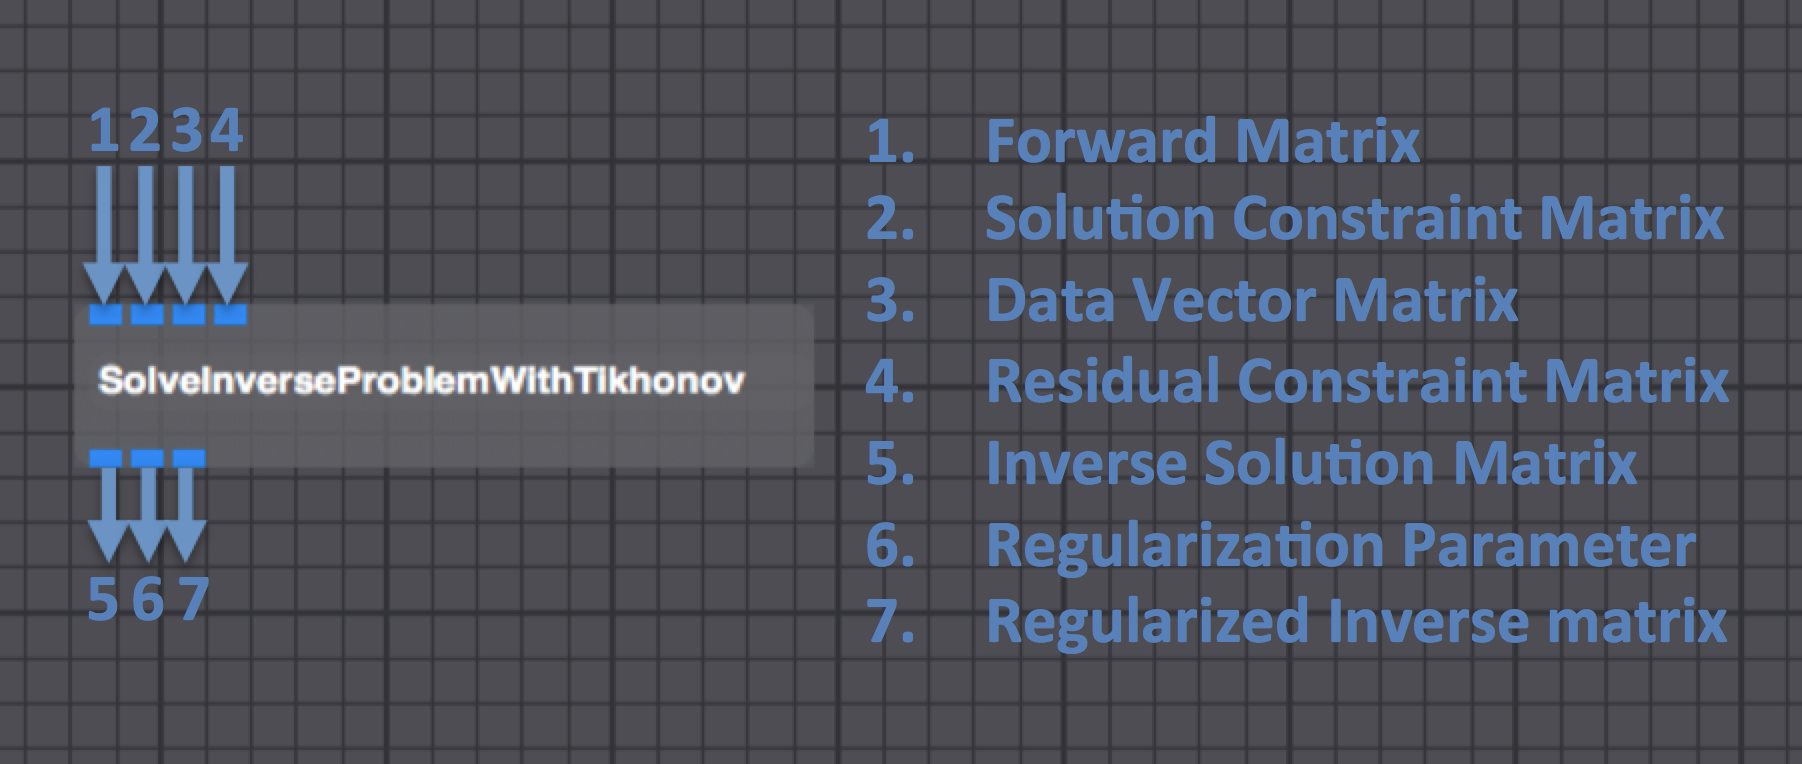
\includegraphics[width=0.7\textwidth]{ECGToolkitGuide_figures/tik1.png}
        \caption{Revised Tikhonov module: {\tt SolveInverseProblemWithTikhonov}.  }
        \label{fig:tik_module}
        \end{center}
    \end{figure}
    \noindent{\bf Inputs:}
    \begin{enumerate}
        \item Forward Matrix ($A\in\Re^{N,M}$)
        \item Weights in Source Space ($R\in\Re^{L,M}$ or squared $R^2\in\Re^{M,M}$ o)
        \item Measured Potentials ($Y\in\Re^{N,T}$)
        \item Weights in Sensor Space ($P\in\Re^{F,N}$ or squared $P^2\in\Re^{N,N}$),
    \end{enumerate}
    {\bf Outputs:}
     \begin{enumerate}
        \item Inverse Solution ($X\in\Re^{M,T}$)
        \item Regularization Parameter ($\lambda$)
        \item Regularized Inverse ($G\in\Re^{M,N}$)
    \end{enumerate}

    An example of the usage of the module \href{http://scirundocwiki.sci.utah.edu/SCIRunDocs/index.php/CIBC:Documentation:SCIRun:Reference:BioPSE:SolveInverseProblemWithTikhonov}{{\tt SolveInverseProblemWithTikhonov}} can be found in the network ``potential-based-inverse/tikhonov-inverse.srn5'', which is shown in \autoref{TikhonovNetworkExample}.
    This example network is composed of four main blocks:
    \begin{itemize}
        \item {\bf Loading Data (green):} These are the modules that load the data into SCIRun.
        \item {\bf Forward Solution (white):} These modules compute simulations of ECG potentials that would be measured on the body surface.
        \item {\bf Tikhonov Inverse (black):} This module computes the Tikhonov inverse solution.
        \item {\bf Visualization (purple):} These modules provide visualization of the solution and the ground truth.
    \end{itemize}
    
    \subsubsection{Options and Modes of Operation}
    
    The \href{http://scirundocwiki.sci.utah.edu/SCIRunDocs/index.php/CIBC:Documentation:SCIRun:Reference:BioPSE:SolveInverseProblemWithTikhonov}{{\tt SolveInverseProblemWithTikhonov}} module allows for multiple modes of operation that provide different functionalities and computational advantages.
    These modes of operation, can be found in the two panels of the module user interface, shown in \autoref{fig:tik_module_gui}. 
    The options within each of the two panels are described in the following:
    
    \begin{figure}
    \begin{center}
    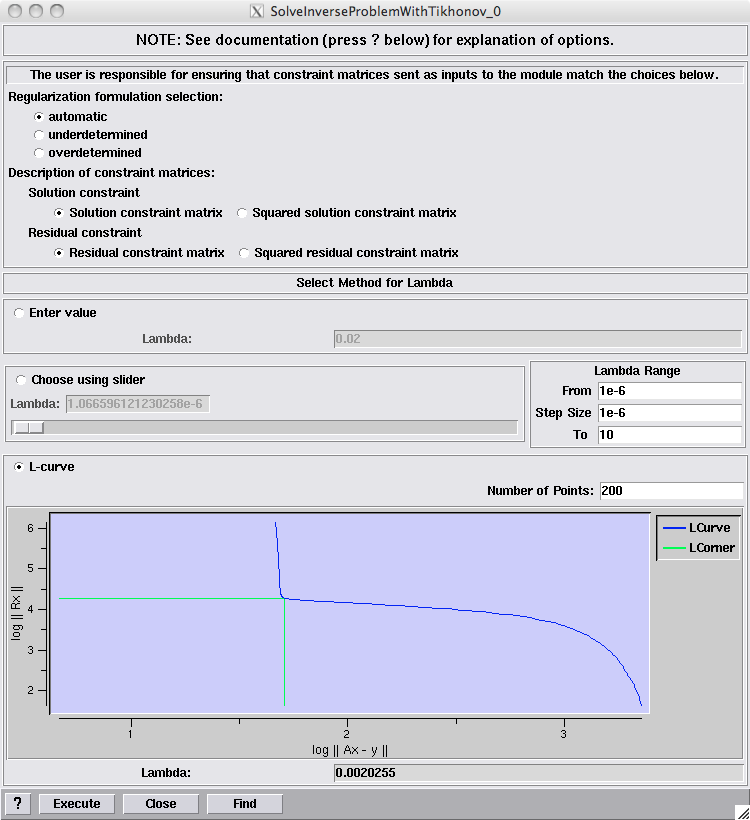
\includegraphics[width=0.45\textwidth]{ECGToolkitGuide_figures/tik2.png}
    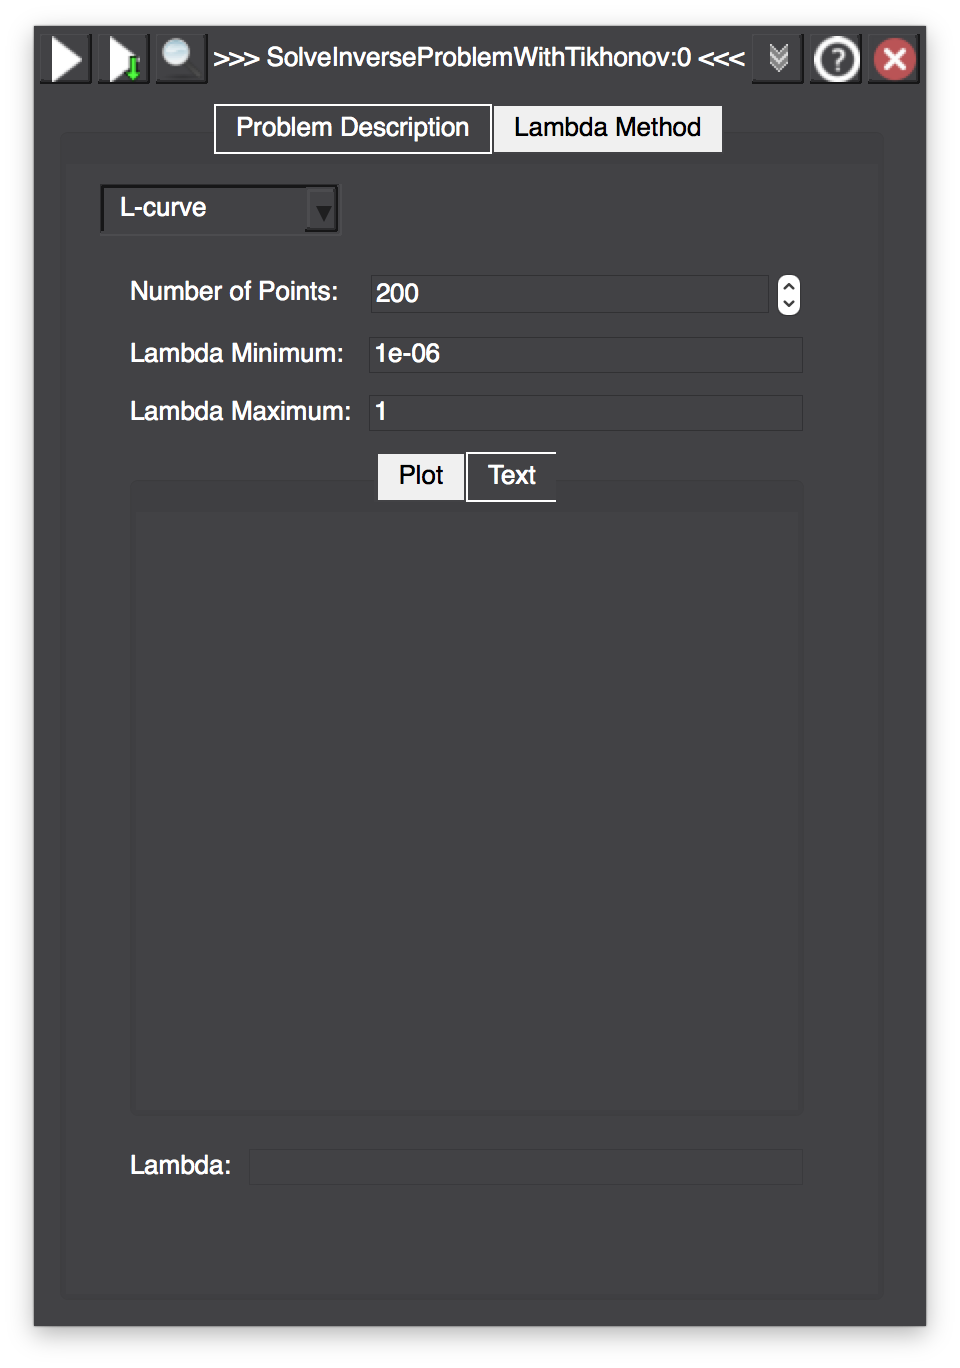
\includegraphics[width=0.45\textwidth]{ECGToolkitGuide_figures/tik3.png}
    \caption{GUI from revised Tikhonov module. Left: problem description. Right: Lambda selection method {\tt SolveInverseProblemWithTikhonov}.}
    \label{fig:tik_module_gui}
    \end{center}
    \end{figure}

    \noindent{\bf Problem Description:}
    
    There are two formulations for the solutions of least squares problem in \autoref{eq:inverseSec_tik_problem}.
    These are the overdetermined formulation:
    \begin{center}
    \begin{eqnarray}
        \hat{x}   &=& \left(A^T P^TPA + \lambda^{2}R^TR\right)^{-1} A^T P^TP y,
    \label{eq:inverseSec_TikhonovSolutions1}
    \end{eqnarray}
    \end{center}    
    and the underdetermined:
    \begin{center}
    \begin{eqnarray}
        \hat{x}  &=& (R^TR)^{-1} A^T \left( A(R^TR)^{-1}A^T + \lambda^2 (P^TP)^{-1}  \right)^{-1}y.
    \label{eq:inverseSec_TikhonovSolutions2}
    \end{eqnarray}
    \end{center}
    The difference between these two formulations is computational. 
    It can be observed from equations \ref{eq:inverseSec_TikhonovSolutions1} and \ref{eq:inverseSec_TikhonovSolutions2} that the size of the inverse matrix that needs to be computed is $N$ in the overdetermined case and $M$ in the underdetermined.
    Thus, when the number of ECG measurements is smaller than the number of sources on the heart ($N<M$), it is computationally desirable to use \autoref{eq:inverseSec_TikhonovSolutions1}.
    On the other hand, if the number of ECG measurements is larger than the number of sources ($N>M$), it is preferable to use \autoref{eq:inverseSec_TikhonovSolutions2}.
    \href{http://scirundocwiki.sci.utah.edu/SCIRunDocs/index.php/CIBC:Documentation:SCIRun:Reference:BioPSE:SolveInverseProblemWithTikhonov}{{\tt SolveInverseProblemWithTikhonov}} is prepared to use either formulation upon request of the user or choose it automatically based on the size of the forward matrix.
    To choose the desired option, the user must select the appropriate radial button in the ``Regularization Formulation'' option within the  ``Problem Description'' panel.
    
    The ``Problem Description'' panel also allows to modify how the source and sensor weight matrices ($R$ and $P$) are defined.
    As can be observed in equations \ref{eq:inverseSec_TikhonovSolutions1} and \ref{eq:inverseSec_TikhonovSolutions2}, these two matrices appear in quadratic form. For this reason, many users might prefer to define them in the quadratic form (i.e. $R^2=R^TR$ and $C^2=C^TC$).
    \href{http://scirundocwiki.sci.utah.edu/SCIRunDocs/index.php/CIBC:Documentation:SCIRun:Reference:BioPSE:SolveInverseProblemWithTikhonov}{{\tt SolveInverseProblemWithTikhonov}} allows users to change the default definition of these input matrices to the squared form by selecting the appropriate radial buttons in the ``Constraint Matrices'' options within the  ``Problem Description'' panel.
    
    
    \noindent{\bf Lambda Method:}
    
    The solutions to the Tikhonov regularization problem depend on the selection of the regularization parameter ($\lambda$).
    There are multiple approaches in the literature that allow for its selection.
    \href{http://scirundocwiki.sci.utah.edu/SCIRunDocs/index.php/CIBC:Documentation:SCIRun:Reference:BioPSE:SolveInverseProblemWithTikhonov}{{\tt SolveInverseProblemWithTikhonov}} is currently implemented so that the user can choose between a direct entry, selection using a slider and the L-curve method, described in \autoref{sec:math:regparam}.
    These methods can be found by selecting the appropriate option in the drop-down menu within the ``Lambda Method'' panel.
    
    
    \begin{figure}
        \begin{center}
        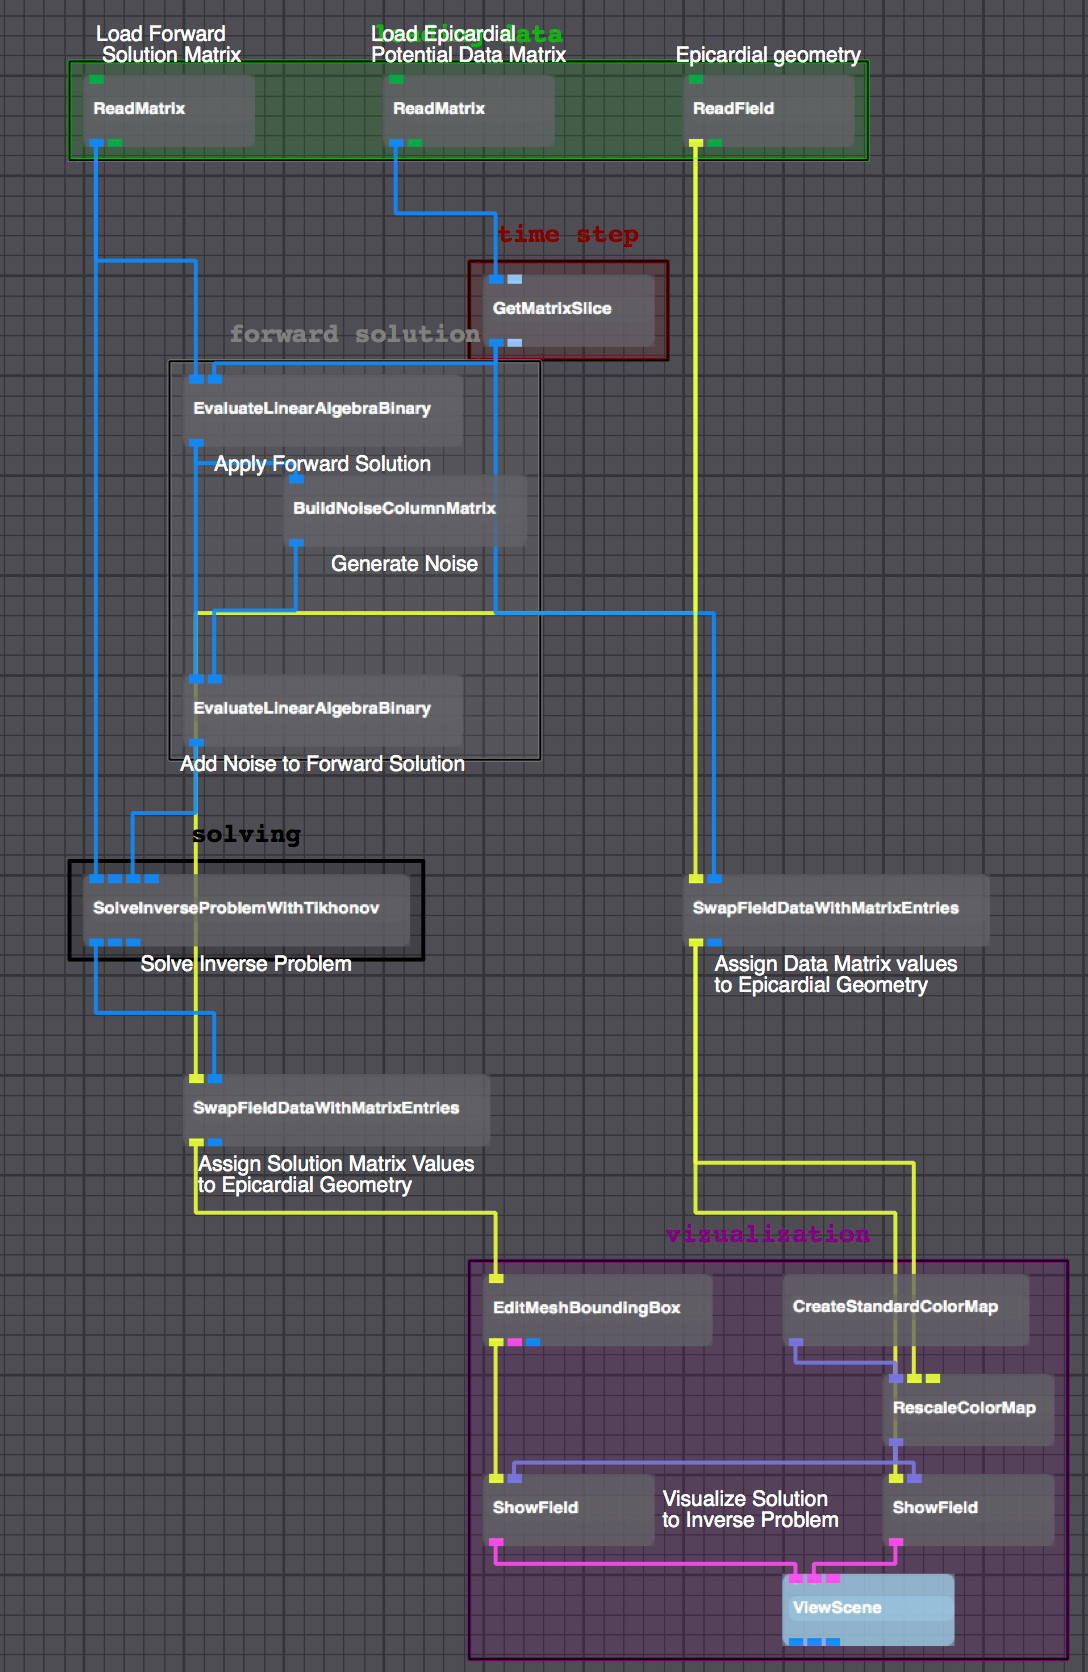
\includegraphics[width=0.9\textwidth]{ECGToolkitGuide_figures/TikhonovNetwork.png}
        \caption{The SCIRun network for the Tikhonov inverse solution example.}
        \label{TikhonovNetworkExample}
        \end{center}
    \end{figure}
    
    
\subsection{Tikhonov SVD Method}
    The Tikhonov SVD method effectively solves the same least squares problem as the Tikhonov method described above.
    The difference between these two implementations is computational. 
    The \href{http://scirundocwiki.sci.utah.edu/SCIRunDocs/index.php5/CIBC:Documentation:SCIRun:Reference:BioPSE:SolveInverseProblemWithTikhonovSVD}{{\tt SolveInverseProblemWithTikhonovSVD}} module uses the following formulation to solve the least-squares problem:
    \begin{center}
    \begin{eqnarray}
        \hat{X}   &=& \sum_{k=1}^K \frac{\sigma_k}{\lambda^2 + \sigma_k^2} v_k u_k^T Y,
    \label{eq:inverseSec_TikhonovSolutions1}
    \end{eqnarray}
    \end{center} 
    where $Y$ are the ECG measurements, $X$ are the unknown potentials on the heart, $\lambda$ is the regularization parameter and $\sigma_k$, $u_k$ and $v_k$ are the singular values and left and right singular vectors of the forward matrix $A$.
    
    The \href{http://scirundocwiki.sci.utah.edu/SCIRunDocs/index.php5/CIBC:Documentation:SCIRun:Reference:BioPSE:SolveInverseProblemWithTikhonovSVD}{{\tt SolveInverseProblemWithTikhonovSVD}} module is shown in \autoref{fig:tik_moduleSVD}.
    \begin{figure}
        \begin{center}
        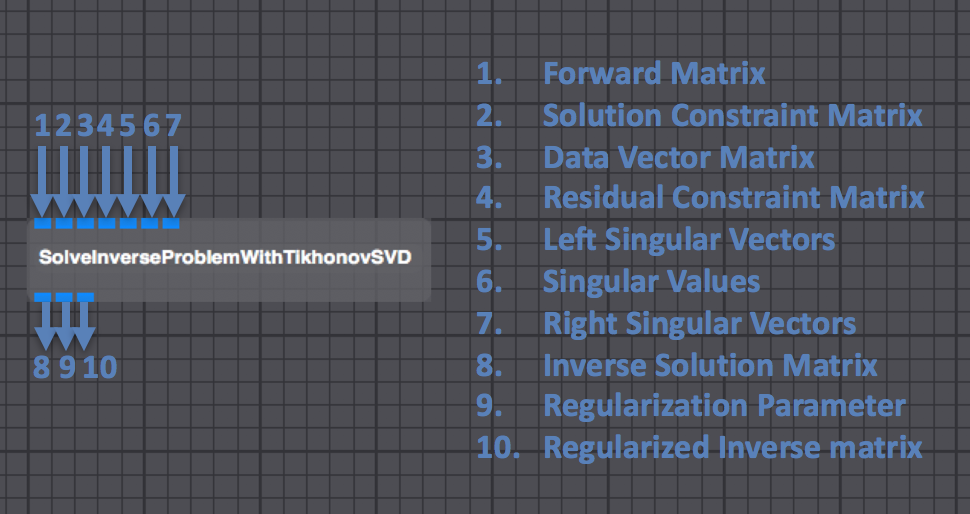
\includegraphics[width=0.7\textwidth]{ECGToolkitGuide_figures/TikhonovSVD_module.png}
        \caption{Revised TikhonovSVD module: {\tt SolveInverseProblemWithTikhonovSVD}.  }
        \label{fig:tik_moduleSVD}
        \end{center}
    \end{figure}
    The inputs and outputs of this module are a superset of \href{http://scirundocwiki.sci.utah.edu/SCIRunDocs/index.php/CIBC:Documentation:SCIRun:Reference:BioPSE:SolveInverseProblemWithTikhonov}{{\tt SolveInverseProblemWithTikhonov}}.
    The new additions permit the user to use pre-computed singular values and vectors of the forward matrix.
    \noindent{\bf Inputs:}
    \begin{enumerate}
        \item Forward Matrix ($A\in\Re^{N,M}$)
        \item Weights in Source Space ($R\in\Re^{L,M}$ or squared $R^2\in\Re^{M,M}$ o)
        \item Measured Potentials ($Y\in\Re^{N,T}$)
        \item Weights in Sensor Space ($P\in\Re^{F,N}$ or squared $P^2\in\Re^{N,N}$)
        \item Left Singular Vectors ($U\in\Re^{N,N}$ )
        \item Singular Values ($S\in\Re^{K,K}$ or in vector form $s\in\Re^{K,1}$)
        \item Right Singular Vectors ($V\in\Re^{M,M}$),
    \end{enumerate}
    {\bf Outputs:}
     \begin{enumerate}
        \item Inverse Solution ($X\in\Re^{M,T}$)
        \item Regularization Parameter ($\lambda$)
        \item Regularized Inverse ($G\in\Re^{M,N}$)
    \end{enumerate}
    
    \subsubsection{Options and Modes of Operation}
    
    The options allowed in \href{http://scirundocwiki.sci.utah.edu/SCIRunDocs/index.php5/CIBC:Documentation:SCIRun:Reference:BioPSE:SolveInverseProblemWithTikhonovSVD}{{\tt SolveInverseProblemWithTikhonovSVD}} include the use of a pre-computed singular value decomposition of the forward matrix and the method to select the regularization parameter $\lambda$.
    
    \noindent{\bf Pre-computed Singular Value Decompositions}
    
    When needed, \href{http://scirundocwiki.sci.utah.edu/SCIRunDocs/index.php5/CIBC:Documentation:SCIRun:Reference:BioPSE:SolveInverseProblemWithTikhonovSVD}{{\tt SolveInverseProblemWithTikhonovSVD}} automatically computes a Singular Value Decomposition of the input forward matrix using sub-routines found in the Eigen library.
    However, the module is also prepared to use a pre-computed singular value decomposition. 
    This option is selected by connecting ALL the input ports of the left and right singular vectors and singular values (ports 5, 6 and 7).
    In this case, the algorithm skips the computation of the SVD and uses the provided matrices.
    
    \noindent{\bf Lambda Method}
    
    The solutions to the TikhonovSVD regularization problem depend on the selection of the regularization parameter ($\lambda$).
    There are multiple approaches in the literature that allow for its selection.
    \href{http://scirundocwiki.sci.utah.edu/SCIRunDocs/index.php5/CIBC:Documentation:SCIRun:Reference:BioPSE:SolveInverseProblemWithTikhonovSVD}{{\tt SolveInverseProblemWithTikhonovSVD}} is currently implemented so that the user can choose between a direct entry, selection using a slider and the L-curve method, described in \autoref{sec:math:regparam}.
    These methods can be found by selecting the appropriate option in the drop-down menu within the ``Lambda Method'' panel as done in \href{http://scirundocwiki.sci.utah.edu/SCIRunDocs/index.php/CIBC:Documentation:SCIRun:Reference:BioPSE:SolveInverseProblemWithTikhonov}{{\tt SolveInverseProblemWithTikhonov}} (see \autoref{fig:tik_module_gui}).
    
    
    \begin{figure}
        \begin{center}
        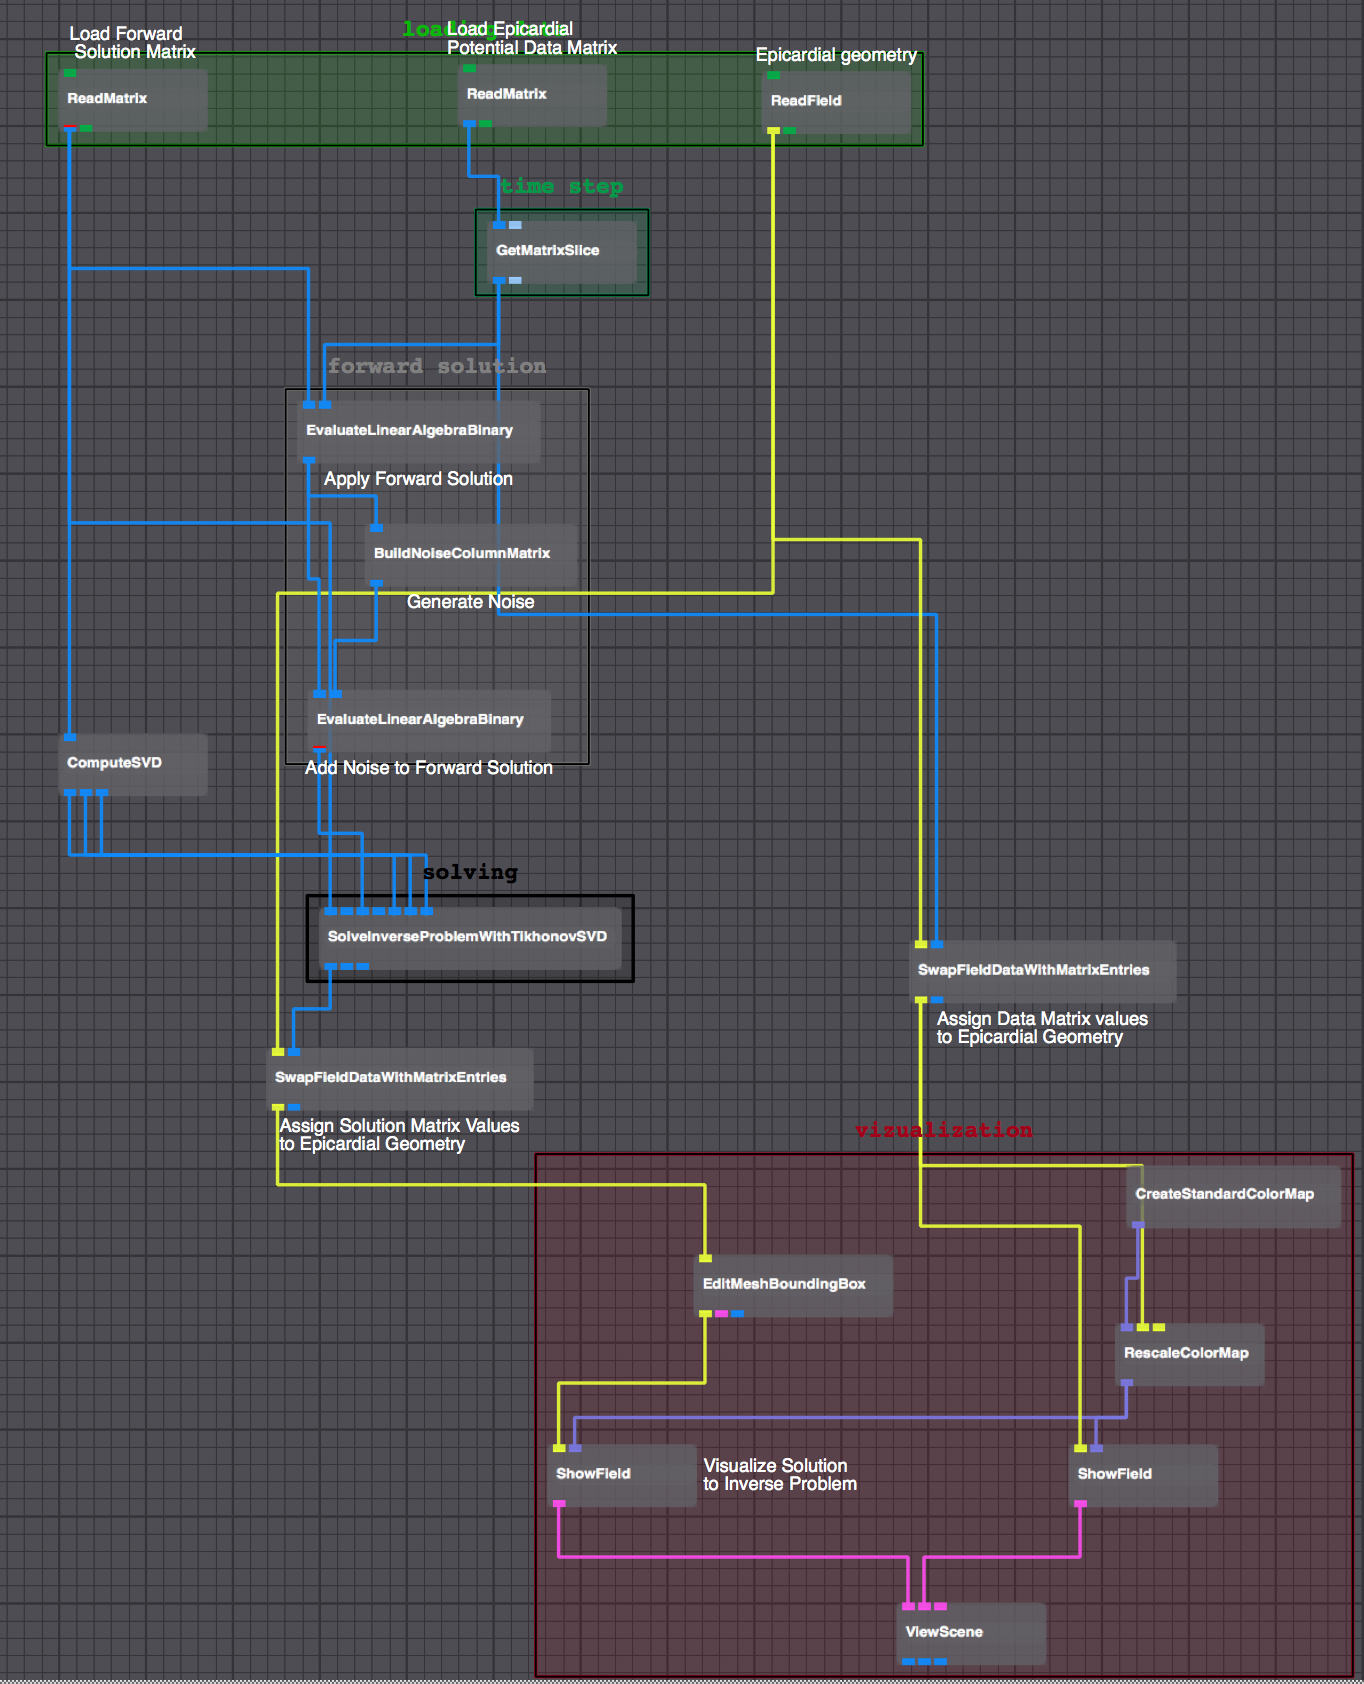
\includegraphics[width=0.9\textwidth]{ECGToolkitGuide_figures/TikhonovSVDNetwork.png}
        \caption{The SCIRun network for the TikhonovSVD inverse solution example.}
        \label{fig:TikhonovNetworkExampleSVD}
        \end{center}
    \end{figure}
    
\subsection{Truncated SVD Method (TSVD)}
    
    \subsubsection{Options and Modes of Operation}

\subsection{Method of Fundamental Solutions}

\subsection{Isotropy Method}

\subsection{Spline-Based Inverse Method}

\subsection{Activation-Based Method}

\subsection{Wavefront-Based Potential Reconstruction (WBPR)}


\newpage

%%%%%%%%%%%%%%%%%%%%%%%
\subsection{Truncated SVD}

\begin{figure}[H]
\begin{center}
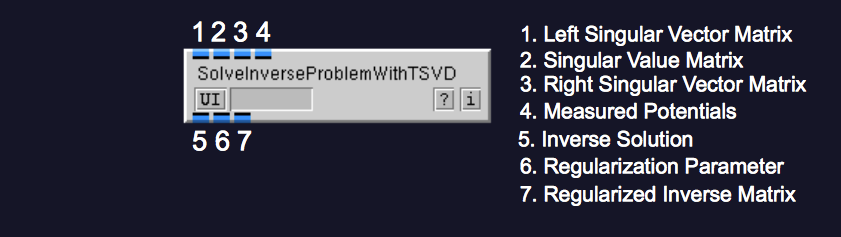
\includegraphics[width=\textwidth]{ECGToolkitGuide_figures/SolveInverseProblemWithTSVD.png}
\caption{Truncated SVD Module}
\label{tsvd}
\end{center}
\end{figure}

\vspace{5pt}\textit{This is a method of solving the potential-based inverse problem.}\vspace{5pt}

This module, called {\tt SolveInverseProblemWithTSVD}, computes an inverse solution by creating a pseudo-inverse operator and multiplying that with the measured body surface potentials. The module requires that the SVD of a forward solution matrix (left/right singular vector matrices and singular value matrix) and a vector of observed/measured body surface potentials are supplied as input.

In the user interface (UI), one can explicitly specify a scalar-integer regularization parameter to control the amount of regularization imposed on the problem. Assuming the singular values are sorted from largest to smallest (and therefore most significant to least significant), the regularization parameter controls how many significant singular values to consider (truncation degree) when calculating the pseudo-inverse. Alternatively, the module will use the L-curve method to automatically obtain a suitable truncation degree.

The primary output of this module is a vector containing the inverse solution. In addition, it will output the regularization parameter and regularized inverse operator used to obtain the inverse solution from the measured body surface potentials.

%%%%%%%%%%%%%%%%%%%%%%%%%

\subsection{Matlab Interface}

The \textit{InterfaceWithMatlab} module allows a SCIRun network to make use of Matlab for some of its calculations. In Figure \ref{matlabinterfacemodule}, the user interface for this module shows how SCIRun data types from the module's input pipes are converted to Matlab variables for use in a Matlab script. Upon completion of the Matlab script, Matlab variables are converted back to SCIRun data types to be sent to the module's output pipes.

\begin{figure}[H]
\begin{center}
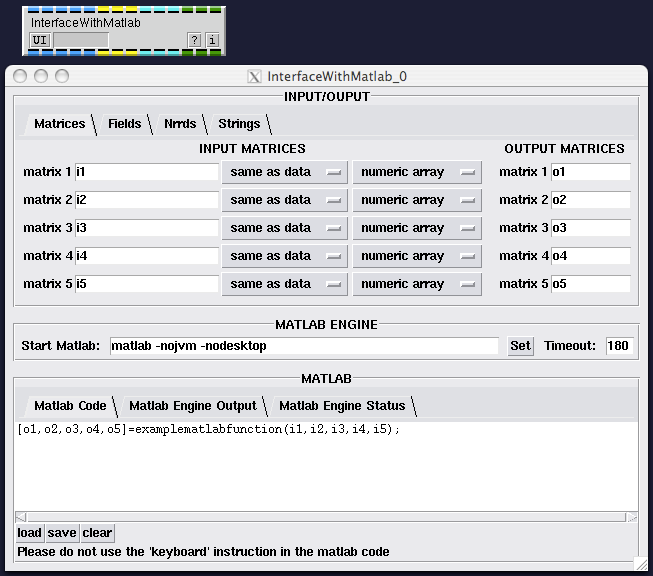
\includegraphics[width=0.8\textwidth]{ECGToolkitGuide_figures/InterfaceWithMatlab.png}
\caption{The InterfaceWithMatlab Module and its corresponding user interface}
\label{matlabinterfacemodule}
\end{center}
\end{figure}

In the rest of this section, we will describe some of the inverse solution methods distributed with SCIRun that have been implemented in Matlab.


\subsubsection{Isotropy Method}

\vspace{5pt}\textit{This is a method of solving the potential-based inverse problem.}\vspace{5pt}

\begin{verbatim}
function X_reg=greensite(A,Y,trunc_deg)
% Function to calculate the Greensite inverse solution
%   A - forward matrix
%   Y - data
%   trunc_deg - truncation degree
%   X_reg - inverse solution
\end{verbatim}

The isotropy method (a.k.a. Greensite method) takes as input a forward solution matrix, measured body surface potential data, and an optional integer regularization parameter (truncation degree). In this method, the truncation degree controls the number of significant singular values of the measured body surface potential data to be used when computing the inverse solution. Consequently, the truncation degree partitions the measured body surface potential data into independent ``signal'' and ``noise'' components, ignoring the ``noise'' component in its calculation of the inverse solution. The only output of the method is the inverse solution.

\subsubsection{Gauss-Newton Method}

\vspace{5pt}\textit{This is a method of solving the activation-based inverse problem.}\vspace{5pt}

\begin{verbatim}
function tau = ActGaussNewton(A,Y,L,tauinit,lambda,w,minstep)
% Implements the Gauss-Newton algorithm for solving the activation-based
% inverse problem of electrocardiography.
% => minimizes the objective function ||Y-A*X||^2+lambda*||L*X||^2 where
% X is parameterized by the C^1 polynomial approximation to a step function
% as explained in "The Depolarization Sequence of the Human Heart Surface
% Computed from Measured Body Surface Potentials" by Geertjan Huiskamp and
% Adriaan van Oosterom.
%
% Input Variables:
% A: Forward matrix
% Y: Observations (columns index time from 1 to T=size(Y,2))
% L: Regularization matrix (typically a surface Laplacian approximation)
% lambda: Regularization parameter
% w: Width parameter in step function approximation
% tauinit: Initial phase shifts for starting the algorithm
%
% Output Variables:
% tau: Solution phase shifts of the step functions
\end{verbatim}

The activation-based inverse problem of electrocardiography is to solve for electrical activation times (i.e. depolarization times) on the heart, given body surface potentials during the QRS complex. This results in a nonlinear least-squares optimization problem that this method solves using the Gauss-Newton algorithm. Solutions are typically highly dependent on the choice of the initial guess. This method requires a forward solution matrix, body surface potentials, regularization matrix, initial guess, regularization parameter, activation waveform transition width, and convergence parameter to be specified as input. The body surface potentials should be provided as a $M \times T$ matrix, where $M$ is the number of leads from which potentials are recorded and $T$ is the number of time samples recorded during the QRS complex of the heart, whose activation times are to be estimated. The regularization matrix and corresponding parameter influence the inverse solution as in Tikhonov regularization (see above). The initial guess is the set of activation times from which the Gauss-Newton algorithm starts pursuing a more suitable inverse solution. The transition width controls the number of time samples (not necessarily integer) taken by each source to transition from inactivated to activated in this method. The convergence parameter is the minimum norm of the step taken by the iterations within the Gauss-Newton algorithm before the method is deemed to have converged to a suitable solution. The only output of the method is the inverse solution (in this case: an array/vector of activation times).

\subsubsection{Wavefront-Based Potential Reconstruction}

\vspace{5pt}\textit{This is a method of solving the potential-based inverse problem.}\vspace{5pt}

\begin{verbatim}
function [x_WBPR_forward,x_WBPR_backward] = WBPR(A,y,heart,first_act,last_act)
% Function to calculate the WBPR solutions
% Inputs:
%   A: forward matrix
%   y: torso data
%   heart: heart geometry
%   first_act: first activated node
%   last_act: last activated node
%
% Outputs:
%   x_WBPR_forward: inverse solution using forward WBPR
%   x_WBPR_backward: inverse solution using backward WBPR
\end{verbatim}

The Wavefront-Based Potential Reconstruction (WBPR) method imposes prior knowledge about the spatial patterns of electric potentials on the heart during the QRS complex to reconstruct an inverse solution. This method requires a forward solution matrix, measured body surface potentials, a structure containing the triangles and nodes of the heart geometry mesh, and the first/last nodes to activate during the QRS complex of the heart beat. The body surface potentials should be provided as a $M \times T$ matrix, where $M$ is the number of leads from which potentials are recorded, and $T$ is the number of time samples recorded during the QRS complex of the heart beat, whose electric potentials are to be estimated. The heart geometry is a Matlab ``struct'' that must contain a matrix of node coordinates and a matrix of indices for triangles that connect the nodes on the surface of the heart. The first/last nodes to activate are specified as the indices of the nodes.

As output, WBPR produces two inverse solutions. The procedure by which the inverse solutions are obtained may be run both forward and backward in time. Therefore, the ``forward WBPR'' solution is that obtained by applying the method starting from the earliest sample time and ending at the latest. On the other hand, the ``backward WBPR'' solution is obtained by starting from the latest sample time and traversing the samples in reverse until ending at the earliest.

NOTE: This code requires the software package reguTools (http://www.imm.dtu.dk/~pcha/Regutools/) to be incorporated in the default path from MATLAB.


\subsubsection{Non-Negative Transmembrane Potential Inverse}

\vspace{5pt}\textit{This is a method of solving the potential-based inverse problem.}\vspace{5pt}
\begin{verbatim}
%% MESSNARZ INVERSE SCRIPT FOR SCIRUN
%
%		This is a script for the matlab interface in the SCIRUN network
%		nonNegative.srn.
%		This method consists in a potential based inverse method that 
%		uses tikhonov reularization in a minimization algorithm that 
%		constrains the solutions to be monotonically non-decreasing.
%		
%			Inputs:
%				   i1 - double - primal/dual tradeoff parameter from the ADMM algorithm.
%				   i2 - <N,T>double - ECG recordings. (N leads, T time samples)
%				   i3 - <N,M>double - forward matrix.
%				   i4 - <1,3>int - lambda parameters: [minLam maxLam numLam].
%			                           minLam - minimum lambda = 10^minLam
%			                           maxLam - maximum lambda = 10^maxLam
%			                           numLam - number of lambdas to use 
%			Outputs::
%				   o1 - <M,T>double - estimated solution.
%				   o2 - <M,T+1>double - dual variables of ADMM code.
%
\end{verbatim}

The non-negativeTMP code estimates the transmembrane potentials by solving a constrained Tikhonov problem.
Thus the function to be optimized over is a standard Tikhonov problem but restricts the solutions to always be non-decreasing.
Thus, the problem to be solved is:
\begin{equation}\begin{split}
		\min_{x(t), t=1\dots T} &\|y(t) - Ax(t)\|_2^2 + \lambda*\|Rx(t)\|_2^2 \\
		&s.t.\\
   		&\hspace{2cm}x(1) >= minB\\
     	&\hspace{2cm}x(t+1) >= x(t), \hspace{.2cm}t=1\dots T-1\\
     	&\hspace{2cm}x(T) <= maxB
\end{split}
\end{equation}
Where $minB$ and $maxB$ are the minimum and maximum bounds for the TMP.
For memory efficiency, this problem is implemented with an ADMM solver.
This algorithm tends to work well for relatively small geometries ($<1000$ nodes).
The resulting potentials have sharp increases of potentials similar to the typically observed in TMPs 
for most of the nodes on the heart geometry.
In general, the final solution is insensitive to the initial guess but it will affect the time of convergence.
The script is set up such that the initial guess for the first lambda is a simple ramp, after each initial guess is the final result of the previous lambda. 
The decision of the correct lambda is done automatically using an L-corner detection.
This algorithm is implemented as the SCIRUN network nonNegativeTMP.srn

NOTE: This code requires the software package reguTools (http://www.imm.dtu.dk/~pcha/Regutools/) to be incorporated in the default path from MATLAB.

\subsubsection{Spline Interpolation Inverse}

\vspace{5pt}\textit{This is a method of solving the potential-based inverse problem.}\vspace{5pt}
\begin{verbatim}
%		This code implements the inverse solutions pipeline presented in
%		the paper:
%	        Erem, Coll-font, Martinez Orellana - 2013 - 
%	        Using Transmural Regularization and Dynamic Modeling 
%	        for Non-Invasive Cardiac Potential Imaging of 
%	        Endocardial Pacing Sites with Imprecise Thoracic Geometry.
%
%		Inputs
%				  i1 - <N,T>double - measured potentials on the torso.
%				  i2 - <N,M>double - forward matrix.
%				  i3 - <L,M>double - regularization matrix.
%				  i4 - <3,1>int - regularization constant params.
%				                  i4(1) - log10 min lambda.
%				                  i4(2) - log10 max lambda
%				                  i4(3) - num lambda.
%		Outputs
%				  o1 - <M,T>double - estimated heart potentials.
\end{verbatim}

This code implements a spline interpolation based inverse for ECG.
It works under the assumption that the measured cardiac potentials, treated as a vector in high dimensional space, span a 1-D manifold in time.
This algorithm approximates this manifold with a spline, effectively filtering out noise to describe the evolution of these potentials.
Then it estimates the inverse of the reference points (knot points) of the spline and reconstructs the full evolution of potentials in the heart using the time dynamics from the body surface potentials.
This algorithm works well when the regularization matrix used in the inverses estimates the spatial derivative in the volume of the heart.
An example of a SCIRUN implementation for this code can be found in the spline$\_$inverse.srn network. 

\subsubsection{Total Variation Inverse}

\vspace{5pt}\textit{This is a method of solving the potential-based inverse problem.}\vspace{5pt}
\begin{verbatim}
%	This script implements a Total Variation method to solve the inverse
%	problem in electrocardiography 
%
%	This code needs of the convex optimization toolbox from CVX
%	(http://cvxr.com/cvx/)
%
%	Inputs:
%    field1 - struct - full bofy geometry.
%    field2 - struct - heart geometry.
%    field3 - struct - torso geometry.
%    i1 - <N,1>double - ECG measured potentials.
%     i2 - <N,1>int - indices of the geometry where ECG where measured.
%    i3 - <M,M>double - stiffness matrix on the heart.
%     i4 - <N+M,N+M>double - stiffness matrix on the whole body.
%	Outputs:
%    o1 - <M,1>double - estimated inverse solution.
%
%	Dependencies:
%    cvx - convex optimization package
%
\end{verbatim}

This code is an implementation of a full pipeline that covers from the solution of the forward problem to an implementation of a Total Variation inverse solution.
This method uses a FEM geometry to calculate the forward matrices needed and then computes the inverse solution from body surface measurements.
The solutions it obtains tend to have sharper spatial transitions that the regular Tikhonov solutions.
An example SCIRUN implementation for this MATLAB implementation is the Total$\_$Variation.srn in the FwdInvToolbox.

NOTE: This code requires the software package CVX (http://cvxr.com/cvx/) for MATLAB to be set up in the default path of MATLAB.

%%%%%%%%%%%%%%%%%%%%%%%%%
\section{Example Simulations}

\subsection{Tikhonov Regularization}

\vspace{5pt}\textit{The SCIRun network for this example can be found at:\\{\tt src/nets/FwdInvToolbox/potential-based-inverse/tikhonov-inversion.srn}\\in the SCIRun source code directory.}\vspace{5pt}


This example shows how to use the {\tt SolveInverseProblemWithTikhonov} module in a SCIRun network to solve a potential-based ECG inverse problem using Tikhonov regularization. Specifically, this example simulates ``measured'' body surface potentials by applying a forward solution and adding pseudorandom noise with a specified signal-to-noise ratio (SNR). The forward solution is obtained by multiplying a known vector of epicardial potential data by a pre-computed forward solution matrix. The simulated measurements and forward solution matrix are the inputs to the {\tt SolveInverseProblemWithTikhonov} module. The regularization parameter of this method is controlled via the user interface (UI) in this example. The output from the module is the inverse solution. This example compares the inverse solution to the known epicardial potentials from which the measurements were simulated. A visualization of both can be seen in the UI of the {\tt ViewScene} module.

\subsection{Gauss-Newton Method}

\vspace{5pt}\textit{The SCIRun network for this example can be found at:\\{\tt src/nets/FwdInvToolbox/activation-based-inverse/actgaussnewton-inversion.srn}\\in the SCIRun source code directory.}\vspace{5pt}

This example shows how to use the {\tt InterfaceWithMatlab} module in a SCIRun network to solve an activation-based ECG inverse problem using the Gauss-Newton method. This example uses the ``normal male'' dataset and geometries from ECGSIM. Specifically, this method compares measured body surface potentials with body surface potentials simulated from activation times. We search the set of possible activation times for ones that minimize the squared error residual between the measured and simulated body surface potentials. The Gauss-Newton method in this example is implemented as a Matlab function and is used in SCIRun via the {\tt InterfaceWithMatlab} module. As a numerical optimization method, Gauss-Newton will look for a local minimizer of the squared error residual starting from a suitable initialization point. In this example, we initialize the method with the activation times reported for the dataset in ECGSIM, but perturbed by noise.

\begin{figure}[H]
\begin{center}
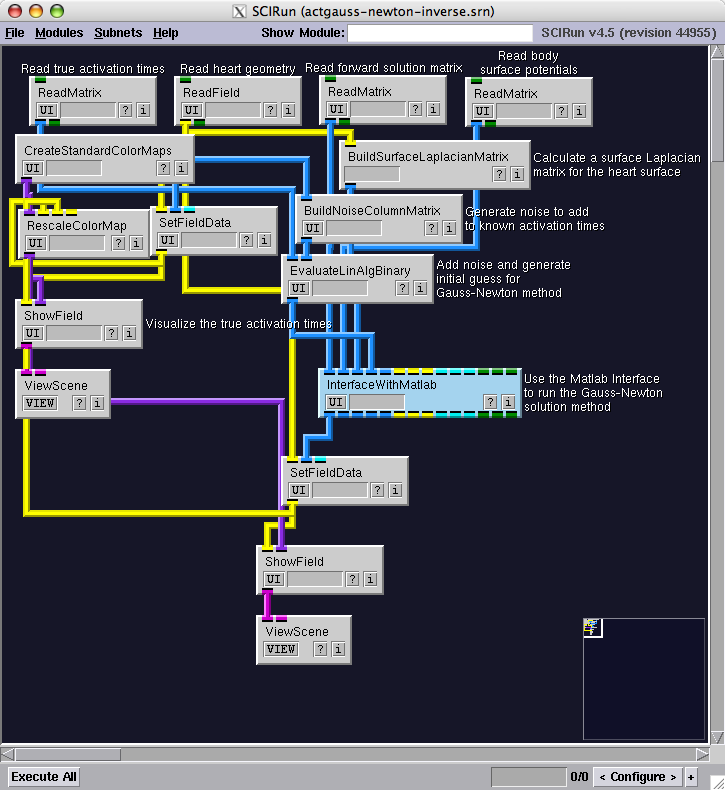
\includegraphics[width=0.9\textwidth]{ECGToolkitGuide_figures/actgaussnewtonnetwork.png}
\caption{The SCIRun network for the activation-based Gauss-Newton inverse solution example.}
\label{GaussNewtonNetworkExample}
\end{center}
\end{figure}

